%%%%%%%%%%%%%%%%%%%%%%%%%%%%%%%%%%%%%%%%%
% University/School Laboratory Report
% LaTeX Template
% Version 3.1 (25/3/14)
%
% This template has been downloaded from:
% http://www.LaTeXTemplates.com
%
% Original author:
% Linux and Unix Users Group at Virginia Tech Wiki 
% (https://vtluug.org/wiki/Example_LaTeX_chem_lab_report)
%
% License:
% CC BY-NC-SA 3.0 (http://creativecommons.org/licenses/by-nc-sa/3.0/)
%
%%%%%%%%%%%%%%%%%%%%%%%%%%%%%%%%%%%%%%%%%

%----------------------------------------------------------------------------------------
%	PACKAGES AND DOCUMENT CONFIGURATIONS
%----------------------------------------------------------------------------------------

\documentclass[12pt]{article}

\usepackage[version=3]{mhchem} % Package for chemical equation typesetting
\usepackage[top=2cm, bottom=2cm, left=3cm, right=2cm]{geometry}%margin defined
\usepackage{siunitx} % Provides the \SI{}{} and \si{} command for typesetting SI units
\usepackage{graphicx} % Required for the inclusion of images
\usepackage{natbib} % Required to change bibliography style to APA
\usepackage{amsmath} % Required for some math elements 
\usepackage[brazil]{babel}% For the portuguese texts
\usepackage[utf8]{inputenc}
\usepackage{float} %for [H] in \begin{figure}[H]
\usepackage{relsize} %for \mathlarger
\setlength\parindent{0pt} % Removes all indentation from paragraphs


\renewcommand{\labelenumi}{\alph{enumi}.} % Make numbering in the enumerate environment by letter rather than number (e.g. section 6)

%definindo novos comandos
\newcommand{\tab}{\hspace{10mm}}
\newcommand{\celsius}{$\,^{\circ}\mathrm{C}$}
\newcommand{\sensibilidade}{\mathlarger{\mathlarger {S}}}

\usepackage{colortbl}%
\newcommand{\myrowcolour}{\rowcolor[gray]{0.925}}
%\usepackage{times} % Uncomment to use the Times New Roman font


%----------------------------------------------------------------------------------------
%	DOCUMENT INFORMATION
%----------------------------------------------------------------------------------------

\title{Trocas de Contexto} % Title
\author{Gabriel Souza e Silva \and Gustavo Cordeiro Libel} % Author name
\date{Abril de 2018} % Date for the report

\begin{document}

\maketitle % Insert the title, author and date
\begin{center}
	Relatório p01
\end{center}

%----------------------------------------------------------------------------------------
%	SECTION 1
%----------------------------------------------------------------------------------------

\section{Funcionamento contexts.c}
Primeiramente o código contextx.c cria as estruturas ucontext\_t ContextPing, ContextPong e ContextMain. Ao iniciar a função main(), é criado um ponteiro do tipo char e o contexto atual é salvo na estrutura ContextPing. Então é alocado espaço para stack e caso esta operação seja executada com sucesso são atribuidos valores para as variáveis de ContextPing, no entanto em caso de erro nesse processo o programa imprime uma messagem de erro e finaliza sua execução.

No caso em que a execução do programa continua, a função makecontext é chamada para alterar o conteúdo de ContextPing. Em seguida, o mesmo procedimento feito com ContextPing é feito com ContextPong. Por fim, na linha 95 a função swapcontext() é chamada para retomar o contexto de ContextPing, executando a função BodyPing que fica alternando contexto com a função BodyPong. Ao fim desse processo, a função swapcontext() é chamada mais uma vez para alterar o contexto para ContextPong e imprimir a ultima mensagem de pong. A saída resultante é a seguinte:

Main INICIO

Ping iniciada

Ping 0

Pong iniciada

Pong 0

Ping 1

Pong 1

Ping 2

Pong 2

Ping 3

Pong 3

Ping FIM

Pong FIM

Main FIM

\textbf{\large ucontext:}

The $<$ucontext.h$>$ header defines the ucontext\_t type as a structure that includes at least the following members:

\begin{table}[H]
	\centering
	%\caption{My caption}
	\label{my-label}
	\begin{tabular}{|l|l|l|}
		\hline 
		ucontext\_t & *uc\_link    & pointer to the context that will be resumed when this context returns \\
		sigset\_t   & uc\_sigmask  & the set of signals that are blocked when this context is active       \\
		stack\_t    & uc\_stack    & the stack used by this context                                        \\
		mcontext\_t & uc\_mcontext & a machine-specific representation of the saved context          \\
		\hline      
	\end{tabular}
\end{table}


\textbf{\large BodyPing/BodyPong:}

print arg e iterador

troca de contexto => Salva o contexto atual em ContextPing e restaura o contexto de ContextPong

faz isso 4 vezes

e troca contexto uma ultima vez

\textbf{\large Main:}

pega contexto
aloca espaço para stack


\section{Chamadas de sistema POSIX para manipulação de contextos.}

	\subsection{int getcontext(ucontext\_t *ucp)}
	A chamada de sistema getcontext é utilizada para receber o contexto em execução no momento, armazenando-o na estrutura apontada por ucp.
	A função retorna 0 em caso de sucesso ou -1 caso o procedimento falhe.
	
	
	\subsection{int setcontext(const ucontext\_t *ucp)}
	A chamada de sistema setcontext restaura o contexto apontado por ucp. Em caso de sucesso, a chamada não retorna algum valor, mas sim retoma o contexto apontado por ucp. Já no caso de falha é retornado -1.
	
	
	\subsection{int swapcontext(ucontext\_t *oucp, ucontext\_t *ucp)}
	A função salva o contexto atual na estrutura apontada por oucp e restaura o contexto armazenado na estrutura apontada por ucp. A função não retorna valores na chamada inicial, no entanto caso o contexto salvo não seja modificado utilizando a função makecontext() e seja feita uma chamada subsequente de setcontext() ou swapcontext() retomando o contexto salvo primeiramente, a função retorna 0.
	
	
	\subsection{void makecontext(ucontext\_t *ucp, void(*func)(), int argc, ...)}
	A função makecontext altera o conteúdo especificado por ucp, que foi inicializado por getcontext() previamente. Quando o contexto é retomado utilizando-se setcontext() ou swapcontext(), a execução do programa continua chamando a função func() passando como argumentos os argumentos que seguem argc na função makecontext().

\section{ucontext\_t.h}
\subsection{ContextPong.uc\_stack.ss\_sp}
Espaço de memória alocado para o contexto.


\subsection{ContextPong.uc\_stack.ss\_size}
Tamanho do espaço de memória alocado para o contexto.


\subsection{ContextPong.uc\_stack.ss\_flags}
É uma variável utilizada para distinguir os casos em que a função getcontext() retorna valores.


\subsection{ContextPong.uc\_link}
Ponteiro para o contexto.


\section*{3. Explicar cada linha do código de contexts.c que chame uma dessas funções ou que manipule estruturas do tipo ucontext\_t .}

\begin{table}[H]
	\centering
	%\caption{My caption}
	\label{my-label}
	\begin{tabular}{|l|l|}
		\hline
		Linhas 26/30  & Salva o contexto atual em ContextPing e restaura o contexto de ContextPong.\\ \myrowcolour
		Linhas 44/48  & Salva o contexto atual em ContextPong e restaura o contexto de ContextPing.\\
		Linha 59      & Salva o contexto atual em ContextPing.  \\ \myrowcolour
		Linha 63 a 67 & \begin{tabular}[c]{@{}l@{}}Ajusta os valores de uc\_stack.ss\_sp, uc\_stack.ss\_size, \\ uc\_stack.ss\_flags, uc\_link de ContextPing.\end{tabular} \\
		Linha 75      & \begin{tabular}[c]{@{}l@{}}Ajusta os valores internos de ContextPing, \\ set função BodyPing e seus argumentos\end{tabular} \\ \myrowcolour
		Linha 77      & Salva o contexto atual em ContextPong. \\
		Linha 82 a 85 & \begin{tabular}[c]{@{}l@{}}Ajusta os valores de uc\_stack.ss\_sp, uc\_stack.ss\_size, \\ uc\_stack.ss\_flags, uc\_link de ContextPong.\end{tabular} \\ \myrowcolour
		Linha 93      & \begin{tabular}[c]{@{}l@{}} Ajusta os valores internos de ContextPong,\\ set função BodyPong e seus argumentos \end{tabular} \\
		Linha 95      & Salva o contexto atual em ContextMain e restaura o contexto de ContextPing.   \\ \myrowcolour
		Linha 96      & Salva o contexto atual em ContextMain e restaura o contexto de ContextPong.    \\ \hline                                                                    
	\end{tabular}
\end{table}

\section*{4. Desenhar o diagrama de tempo da execução}

\begin{figure}[H]

	\begin{center}

		\fbox{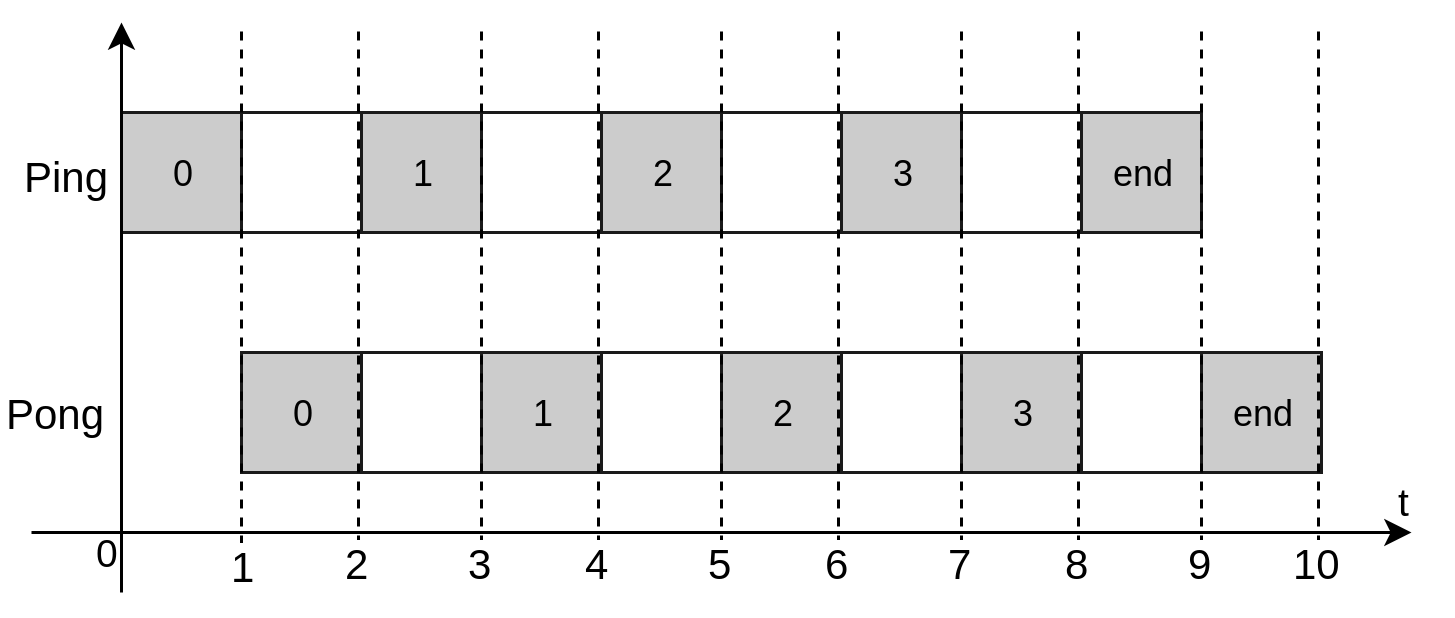
\includegraphics[width=\textwidth]{files/diagrama.png}} % Include the image 

		%\caption{Exorbitante}

		\label{img:diag}

	\end{center}

\end{figure}

\end{document}